\documentclass{beamer}

\mode<presentation>
{
	\usetheme{CambridgeUS}
	\setbeamercovered{transparent}
}
\usepackage[spanish]{babel}
\usepackage[latin1]{inputenc}
\usepackage{color}
\usepackage{hyperref}
\usepackage{multicol}
\usepackage{algorithm,algorithmic}

\title[\textbf{ICI 4242 - Aut\'omatas y compiladores}]{\textbf{ICI 4242 - Aut\'omatas y compiladores}}

\subtitle{An\'alisis Sem\'antico}

\author[Rodrigo Olivares]
{
	Rodrigo Olivares \\
	\vspace{0.5mm}
	Mg. en Ingenier\'ia Inform\'atica \\
	\vspace{0.5mm}
	\texttt{\normalsize rodrigo.olivares@uv.cl}
}

\institute[PUCV]

\date{1er Semestre} 

\subject{An\'alisis Sem\'antico}

%\AtBeginSection
%{
%	\begin{frame}<beamer>
%	\frametitle{Contenido}
%	\tableofcontents[currentsection,currentsubsection]
%	\end{frame}
%}
%
%\AtBeginSubsection
%{
%	\begin{frame}<beamer>
%	\frametitle{Contenido}
%	\tableofcontents[currentsection,currentsubsection]
%	\end{frame}
%}
%
%\beamerdefaultoverlayspecification{<+->}

\begin{document}

	\begin{frame}
		\titlepage
	\end{frame}

%	\begin{frame}
%		\frametitle{Contenido}
%		\tableofcontents[pausesections]
%	\end{frame}

	\section{Funciones del analizador Sem\'antico}

		%\subsection{Definici\'on}

		\begin{frame}
			\frametitle{Funciones del analizador sem\'antico}
			%\framesubtitle{Definici\'on}

			\begin{block}{Definici\'on}
			    El \textbf{Analizador Sem\'antico} es la fase que sigue al an\'alisis sint\'actico. En esta fase se \textbf{explora} el AST (\'arbol de sintaxis abstracta) con el fin de detectar los errores sem\'anticos.
			\end{block}
		\end{frame}

		\begin{frame}
			\frametitle{Funciones del analizador sem\'antico}
			%\framesubtitle{Definici\'on}

			\begin{figure}[H]
			    \begin{center}
			        \fbox{\fbox { 
			            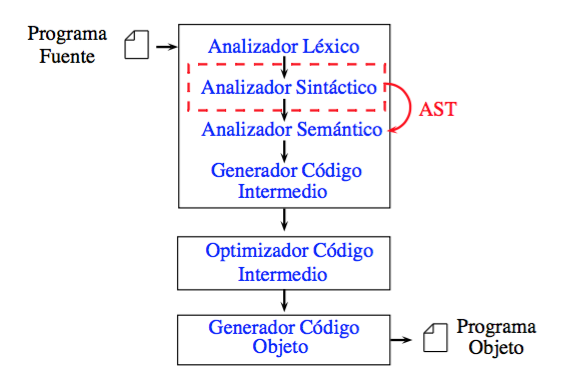
\includegraphics[scale=.45]{images/sin1.png}
			        }}
			    \end{center}
			\end{figure}
		\end{frame}

		\begin{frame}
			\frametitle{Funciones del analizador sem\'antico}

            \begin{block}{}
                \begin{itemize}
                    \item[$\rightarrow$] Interacci\'on con la tabla de s\'imbolos.
                    \begin{itemize}
                        \item[$\rightarrow$] La tabla de s\'imbolos nos permite registrar la informaci\'on de los identificadores declarados en el programa (por ej. variables declaradas).
                    \end{itemize}
                \end{itemize}
            \end{block}
            \begin{block}{}
                 \begin{itemize}
                    \item[$\rightarrow$] Detecci\'on de errores sem\'anticos
                 \end{itemize}
            \end{block}
            \begin{block}{}
                 \begin{itemize}
                    \item[$\rightarrow$] El \textbf{analizador sem\'antico} tambi\'en se conoce como \textbf{tree-parser}.
                 \end{itemize}
            \end{block}
		\end{frame}		

		\begin{frame}
			\frametitle{Implementaci\'on del analizador sem\'antico en ANTLR}
			%\framesubtitle{Definici\'on}

            \begin{block}{}
                \texttt{program} : \#(PROGRAM var\_dec body) SEMICOLON!\\
                \vspace{5pt}
                var\_dec : \#(VAR\_DEC (type id:IDENT {sI.addVar(id);})*) SEMICOLON!\\
                \vspace{5pt}
                type : NUMERIC\_TYPE $|$ STRING\_TYPE SEMICOLON! \\
                \vspace{5pt}
                body : \#(BODY assign) SEMICOLON! \\
                \vspace{5pt}
                assign : IDENT ASSIG expr SEMICOLON! \\
			\end{block}
		\end{frame}

		\begin{frame}
			\frametitle{Implementaci\'on del analizador sem\'antico en ANTLR}
			
			\begin{multicols}{2}
			    \begin{table}[H]
			        \begin{center}
			            \begin{tabular}{l}
			                var \\
			                ~~~~ numeric a; \\
			                begin \\
			                ~~~~ a = (a + 1) * b \\
			                end \\
			            \end{tabular}
			        \end{center}
			    \end{table}
			    \begin{figure}[H]
			    \begin{center}
			        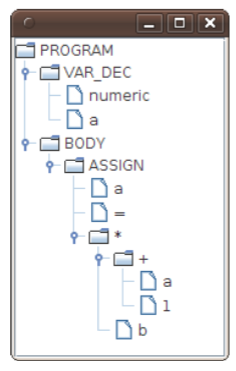
\includegraphics[scale=.55]{images/ast.png}
			    \end{center}
			\end{figure}
			\end{multicols}
	    \end{frame}
	    
		\begin{frame}
			\frametitle{Implementaci\'on del analizador sem\'antico en ANTLR}
			
			\begin{block}{}
			//SemanticInspector.java \\
            $\ldots$ \\
            //Adds the variable to the symbol table \\
            \textbf{public} \textbf{void} addVar(AST var) \{ \\
            \hspace{5pt} \textbf{if}(symbolTable.contains(var.toString())) \\
            \hspace{10pt} \textbf{this}.semanticError(var, `` redefinition of variable ' '' + var + `` ' ''); \\
            \hspace{5pt} \textbf{else} \\
            \hspace{10pt} symbolTable.add(var.toString()); \\
            \} \\
            $\ldots$ \\
            // Checks if the symbol table contains the given variable \\
            \textbf{public} \textbf{void} checkVar(AST var) \{\\
            \hspace{5pt} \textbf{if}(!symbolTable.contains(var.toString()))\\
            \hspace{10pt} \textbf{this}.semanticError(var, `` variable ' '' + var + `` ' is not defined '');\\
            \}
            \end{block}
	    \end{frame}

	    \begin{frame}
			\frametitle{Implemente el analizador sem\'antico del lenguaje MiLe}

			\begin{itemize}
			    \item[$\rightarrow$] Los m\'etodos \textbf{addVar} y \textbf{checkVar} son llamados desde el explorador de \'arboles ANTLR.
			    \item[$\rightarrow$] \textbf{addVar} y \textbf{checkVar} est\'an definidos en \emph{SemanticInspector.java} 
			    \item[$\rightarrow$] \textbf{addVar} agrega variables a la tabla de s\'imbolos, verificando que no hayan sido agregadas previamente.
			    \item[$\rightarrow$] \textbf{checkVar} verifica que la variable ingresada est\'e registrada en la tabla de s\'imbolos.
			\end{itemize}
        \end{frame}

		\begin{frame}
			\frametitle{Preguntas}

			\hspace{4cm}\huge{Preguntas ?}
		
		\end{frame}
	\end{document}

\usetheme{default}
\usetheme{JuanLesPins}
\usetheme{Goettingen}
\usetheme{Szeged}
\usetheme{Warsaw}

\usecolortheme{crane}

\usefonttheme{serif}
\usefonttheme{structuresmallcapsserif}
 